\newcommand{\drawgridrectangle}[4]{%
  \begin{tikzpicture}[scale=#4]
    \pgfmathsetmacro{\ymax}{#1}
    \pgfmathsetmacro{\xmax}{#2}

    % Fill the rectangle
    \fill[#3] (0,0) rectangle (\xmax,\ymax);

    % Draw the border
    \draw[white, line width=#4*3pt] (0,0) rectangle (\xmax,\ymax);


    % Draw vertical grid lines
    \pgfmathsetmacro{\xsteps}{#2}
    \foreach \x in {1,...,\xsteps} {
      \draw[white, line width=#4*3pt] (\x,0) -- (\x,\ymax);
    }

    % Draw horizontal grid lines
    \pgfmathsetmacro{\ysteps}{#1}
    \foreach \y in {1,...,\ysteps} {
      \draw[white, line width=#4*3pt] (0,\y) -- (\xmax,\y);
    }
  \end{tikzpicture}%
}

\newsavebox{\taylorStandard}
\savebox{\taylorStandard}{
  \begin{tikzpicture}
    \matrix [%
    matrix of nodes,%
    ampersand replacement=\&,% to use inside a savebox
    nodes={anchor=center, align=center},%
    column sep=4ex,%
    row sep=1ex,%
    ] (taylor)
    {
      \drawgridrectangle{1}{3}{blue!30}{0.33} \& \drawgridrectangle{1}{2}{blue!30}{0.33} \& \drawgridrectangle{1}{1}{blue!30}{0.33}
      \\[-1.5ex]
      $\vx_0$ \& $\vh_0$ \& $\vg_0$
      \\
      \drawgridrectangle{3}{3}{green!30}{0.33} \& \drawgridrectangle{3}{2}{green!30}{0.33} \& \drawgridrectangle{3}{3}{green!30}{0.33}
      \\[-1.5ex]
      $\{\vx_{1,d}\}$ \& $\{\vh_{1,d}\}$ \& $\{\vg_{1,d}\}$
      \\
      \drawgridrectangle{3}{3}{red!30}{0.33} \& \drawgridrectangle{3}{2}{red!30}{0.33} \& \drawgridrectangle{3}{1}{red!30}{0.33} \& \drawgridrectangle{1}{1}{red!60}{0.33}
      \\[-1.5ex]
      $\{\vx_{2,d}\}$ \& $\{\vh_{2,d}\}$ \& $\{\vg_{2,d}\}$ \& $\sum_d \vg_{2,d}$
      \\
    };

    % draw dependencies
    \pgfmathsetmacro{\K}{3}
    \pgfmathsetmacro{\L}{2}

    \foreach \l in {1,...,\L}{
      \pgfmathsetmacro{\lother}{int(\l+1)}
      \foreach \k in {1,...,\K} {
        \pgfmathsetmacro{\row}{int(2*\k-1)}
        \foreach \kother in {\k,...,\K} {
          \pgfmathsetmacro{\rowother}{int(2*\kother-1)}
          \draw[-Stealth, line width=1pt, white!50!black] (taylor-\row-\l.east) -- (taylor-\rowother-\lother.west);
        }
      }
    }
    \pgfmathsetmacro{\Lstart}{int(\L + 1)}
    \pgfmathsetmacro{\Lend}{int(\L + 2)}
    \pgfmathsetmacro{\rowfinal}{int(2*\K - 1)}
    \draw[-Stealth, line width=1pt, white!50!black] (taylor-\rowfinal-\Lstart.east) -- (taylor-\rowfinal-\Lend.west);
  \end{tikzpicture}
}

\newsavebox{\taylorCollapsed}
\savebox{\taylorCollapsed}{
  \begin{tikzpicture}
    \matrix [%
    matrix of nodes,%
    ampersand replacement=\&,% to use inside a savebox
    nodes={anchor=center, align=center},%
    column sep=4ex,%
    row sep=1ex,%
    ] (taylor)
    {
      \drawgridrectangle{1}{3}{blue!30}{0.33} \& \drawgridrectangle{1}{2}{blue!30}{0.33} \& \drawgridrectangle{1}{1}{blue!30}{0.33}
      \\[-1.5ex]
      $\vx_0$ \& $\vh_0$ \& $\vg_0$
      \\
      \drawgridrectangle{3}{3}{green!30}{0.33} \& \drawgridrectangle{3}{2}{green!30}{0.33} \& \drawgridrectangle{3}{3}{green!30}{0.33}
      \\[-1.5ex]
      $\{\vx_{1,d}\}$ \& $\{\vh_{1,d}\}$ \& $\{\vg_{1,d}\}$
      \\[2ex]
      \drawgridrectangle{1}{3}{red!60}{0.33} \& \drawgridrectangle{1}{2}{red!60}{0.33} \& \drawgridrectangle{1}{1}{red!60}{0.33}
      \\[-1.5ex]
      $\sum_d \vx_{2,d}$ \& $\sum_d \vh_{2,d}$ \& $\sum_d \vg_{2,d}$
      \\[1.1ex]
      \& \&
      \\
    };

    % draw dependencies
    \pgfmathsetmacro{\K}{3}
    \pgfmathsetmacro{\L}{2}

    \foreach \l in {1,...,\L}{
      \pgfmathsetmacro{\lother}{int(\l+1)}
      \foreach \k in {1,...,\K} {
        \pgfmathsetmacro{\row}{int(2*\k-1)}
        \foreach \kother in {\k,...,\K} {
          \pgfmathsetmacro{\rowother}{int(2*\kother-1)}
          \draw[-Stealth, line width=1pt, white!50!black] (taylor-\row-\l.east) -- (taylor-\rowother-\lother.west);
        }
      }
    }
  \end{tikzpicture}
}

\begin{figure*}[!t]
  \centering
  \resizebox{\linewidth}{!}{%
    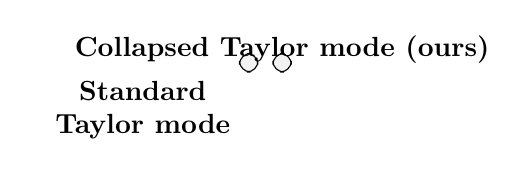
\begin{tikzpicture}
      \node (standard) [fill=black!5!white, draw=black, rounded corners]{\usebox{\taylorStandard}};
      \node [anchor=north east, align=center, inner sep=10pt] at (standard.north east) {\textbf{Standard} \\ \textbf{Taylor mode}};
      \node (collapsed) [fill=black!5!white, draw=black, rounded corners, anchor=north west, xshift=5pt] at (standard.north east) {\usebox{\taylorCollapsed}};
      \node [anchor=south, align=center, inner sep=3pt] at (collapsed.south) {\textbf{Collapsed Taylor mode (ours)}};
    \end{tikzpicture}
  }
  \caption{\textbf{Visual comparison of standard Taylor mode and our proposed collapsed Taylor mode.}}\label{fig:comparison-standard-vs-collapsed}
\end{figure*}

\begin{figure*}
  \centering
  \newsavebox{\taylorStandardNew}
  \savebox{\taylorStandardNew}{
    \begin{tikzpicture}
      \matrix [%
      matrix of nodes,%
      ampersand replacement=\&,% to use inside a savebox
      nodes={anchor=center, align=center},%
      column sep=5ex,%
      row sep=1ex,%
      ] (taylor)
      {
        \drawgridrectangle{1}{5}{gray!25!white}{0.33}
        \& \drawgridrectangle{1}{3}{gray!25!white}{0.33}
        \& \drawgridrectangle{1}{1}{gray!25!white}{0.33}
        \\[-1.5ex]
        $\vx_0$ \& $\vh_0$ \& $\vg_0$
        \\
        \drawgridrectangle{4}{5}{gray!50!white}{0.33}
        \& \drawgridrectangle{4}{3}{gray!50!white}{0.33}
        \& \drawgridrectangle{4}{1}{gray!50!white}{0.33}
        \\[-1.5ex]
        $\{\vx_{1,d}\}$ \& $\{\vh_{1,d}\}$ \& $\{\vg_{1,d}\}$
        \\[0.5ex]
        \drawgridrectangle{1}{5}{white}{0.33}
        \& \drawgridrectangle{1}{3}{white}{0.33}
        \& \drawgridrectangle{1}{1}{white}{0.33}
        \\[0.5ex]
        \\
        \drawgridrectangle{4}{5}{gray}{0.33}
        \& \drawgridrectangle{4}{3}{gray}{0.33}
        \& \drawgridrectangle{4}{1}{gray}{0.33}
        \\[-1.5ex]
        $\{\vx_{K-1,d}\}$ \& $\{\vh_{K-1,d}\}$ \& $\{\vg_{K-1,d}\}$
        \\[0.5ex]
        \drawgridrectangle{4}{5}{red!50}{0.33}
        \&
        \drawgridrectangle{4}{3}{red!50}{0.33}
        \&
        \drawgridrectangle{4}{1}{red!50}{0.33}
        \\[-1.5ex]
        $\{\vx_{K,d}\}$ \& $\{\vh_{K,d}\}$ \& $\{\vg_{K,d}\}$
        \\[-1.5ex]
        \textcolor{purple!50!red}{$\sum_d \vx_{K,d}$}
        \& \textcolor{purple!50!red}{$\sum_d \vh_{K,d}$}
        \& \textcolor{purple!50!red}{$\sum_d \vg_{K,d}$}
        \\
      };

      \node[xshift=-1pt, yshift=-14pt] at (taylor-9-1) {\drawgridrectangle{1}{5}{purple!50!red}{0.33}};
      \node[xshift=-1pt, yshift=-14pt] at (taylor-9-2) {\drawgridrectangle{1}{3}{purple!50!red}{0.33}};
      \node[xshift=-1pt, yshift=-14pt] at (taylor-9-3) {\drawgridrectangle{1}{1}{purple!50!red}{0.33}};

      \node at (taylor-5-1) {\vdots};
      \node at (taylor-5-2) {\vdots};
      \node at (taylor-5-3) {\vdots};

      % draw dependencies
      \pgfmathsetmacro{\K}{5}
      \pgfmathsetmacro{\L}{2}

      \foreach \l in {1,...,\L}{
        \pgfmathsetmacro{\lother}{int(\l+1)}
        \foreach \k in {1,...,\K} {
          \pgfmathsetmacro{\row}{int(2*\k-1)}
          \foreach \kother in {\k,...,\K} {
            \pgfmathsetmacro{\rowother}{int(2*\kother-1)}
            \draw[-Stealth, line width=1pt, gray] (taylor-\row-\l.east) -- (taylor-\rowother-\lother.west);
          }
        }
      }

      \coordinate (arrowStart) at ($(taylor-1-1.north)+(0,3.5ex)$);
      \coordinate (arrowEnd) at ($(taylor-1-3.north east)+(0,3.5ex)$);
      \draw[-Stealth, line width=2pt, black] (arrowStart) to node [midway, fill=white, align=center] {\textbf{Taylor forward} \\ \textbf{propagation}} (arrowEnd);

      \node [left=1.5ex of taylor-1-1] (zero) {0};
      \node [left=1.5ex of taylor-3-1] {1};
      \node [left=1.5ex of taylor-5-1] {$\vdots$};
      \node [left=1.5ex of taylor-7-1] {$K-1$};
      \node [left=1.5ex of taylor-9-1] {$K$};

      \node [align=center] (coefficientLabel) at ($(zero)+(0, 5.5ex)$) {\textbf{Derivative}\\\textbf{degree}};

      \draw[rounded corners] (taylor-9-1.north west) rectangle (taylor.south east);
    \end{tikzpicture}
  }

  \begin{tikzpicture}
    \node {\usebox{\taylorStandardNew}};
  \end{tikzpicture}
\end{figure*}

%%% Local Variables:
%%% mode: LaTeX
%%% TeX-master: "../main"
%%% End:
